\documentclass[a4paper, 12pt]{article}
\usepackage[top=2cm, bottom=2cm, left=2.5cm, right=2.5cm]{geometry}
\usepackage[utf8]{inputenc}
\usepackage[brazilian]{babel}
\usepackage{indentfirst}
\usepackage{graphicx}
\usepackage{wrapfig}
\usepackage[pdftex]{hyperref}
\graphicspath{ {imagens/} }
\usepackage{amsmath}

\begin{document}
%
\begin{titlepage} %iniciando a "capa"
	\begin{center} %centralizar o texto abaixo
		{\large Unicamp}\\[0.4cm] %0,2cm é a distância entre o texto dessa linha e o texto da próxima
		{\large Marco Lucio Bittencourt - Turma B}\\
		{\large Heitor Nigro Lopes - PED}\\[3.2cm]
		{\bf \huge Dinâmica Trabalho 2}\\[0.2cm] 
		{\bf \large Matrizes de Rotação e Range Kutta}\\[4.9cm]
		% o comando \bf deixa o texto entre chaves em negrito. O comando \huge deixa o texto enorme
	\end{center} %término do comando centralizar
	{\large Erik Yuji Goto}\\ % o comando \large deixa o texto grande
	RA: 234009\\[10cm]
	\begin{center}
	
		{\large Campinas}\\[0.2cm]
		{\large 2021}
	\end{center}
\end{titlepage} %término da "capa"


\tableofcontents
\newpage

\section{Matrizes de transformação de coordenadas}
	\subsection{De I para $B_1$}
	\begin{equation}
		T_{\lambda} = \begin{bmatrix}
			cos\alpha && sen\alpha && 0\\
			-sen\alpha && cos\alpha && 0\\
			0 && 0 && 1
		\end{bmatrix}
	\end{equation}
	
	\subsection{De $B_1$ para $B_2$}
	\begin{equation}
		T_{\beta} = \begin{bmatrix}
			cos\beta && sen\beta && 0\\
			-sen\beta && cos\beta && 0\\
			0 && 0 && 1
		\end{bmatrix}
	\end{equation}
	
\section{Velocidade e aceleração angulares absolutas das bases}
	\subsection{Base $B_1$}
	\subsubsection{Velocidade angular}
		\begin{equation}
			\dot{\lambda}^I = \begin{bmatrix}
			0\\0\\ \dot{\lambda}
			\end{bmatrix}
		\end{equation}
	\subsubsection{Aceleração angular}
		\begin{equation}
			\ddot{\lambda}^I = \begin{bmatrix}
			0\\0\\ \ddot{\lambda}
			\end{bmatrix}
		\end{equation}
		
	%Base 2 - aceleração e velocidade angular
	\subsection{Base $B_2$}
	\subsubsection{Velocidade angular}
		\begin{equation}
			\dot{\beta}^{B_1} = \begin{bmatrix}
			0\\0\\ \dot{\beta}
			\end{bmatrix}
		\end{equation}
		\begin{equation}
			\dot{\beta}^{I} = T^T_{\lambda} \dot{\beta}^{B_1} = \begin{bmatrix}
			0\\0\\ \dot{\beta}
			\end{bmatrix}
		\end{equation}
		\begin{equation}
			\dot{\beta}^{I}_{B_2}= \dot{\beta}^{I} + \dot{\lambda}^{I} = \begin{bmatrix}
			0\\0\\ \dot{\beta} + \dot{\lambda}
			\end{bmatrix}
		\end{equation}
	\subsubsection{Aceleração angular}
		\begin{equation}
			\ddot{\beta}^{B_1} = \begin{bmatrix}
			0\\0\\ \ddot{\beta}
			\end{bmatrix}
		\end{equation}
		\begin{equation}
			\ddot{\beta}^{I} = T^T_{\lambda} \ddot{\beta}^{B_1} = \begin{bmatrix}
			0\\0\\ \ddot{\beta}
			\end{bmatrix}
		\end{equation}
		\begin{equation}
			\ddot{\beta}^{I}_{B_2}= \ddot{\beta}^{I} + \ddot{\lambda}^{I} = \begin{bmatrix}
			0\\0\\ \ddot{\beta} + \ddot{\lambda}
			\end{bmatrix}
		\end{equation}
			
			
\section{Vetores de aceleração linear absoluta das massas A e B}
	\subsection{Massa B}
	A aceleração é dada por:
	\begin{equation}
		\vec{a}_B^I = \vec{a}_O^I + \vec{a}_B^{B_1} + \ddot{\lambda}^I \times \vec{r}_{OB}^{I} + \dot{\lambda}^I \times (\dot{\lambda}^I \times \vec{r}_{OB}^{I}) + 2\dot{\lambda}^I \times \vec{v}_B^{B_1}
	\end{equation}
	\begin{itemize}
		\item Vetor posição expresso em relação ao sistema $I$: 
			\begin{equation}
				\vec{r}_{OB}^{B_1} = -l_1 \hat{j} \Rightarrow \vec{r}_{OB}^{I} = T^T_{\lambda}\vec{r}_{OB}^{B_1} = \begin{bmatrix}
			l_1sen \alpha\\
			-l_1cos\alpha\\
			0
		\end{bmatrix}
			\end{equation}					
		

		\item O vetor posição é constante $\Rightarrow \vec{v}_B^{B_1} = \vec{a}_B^{B_1} = 0$
		\item A aceleração do sistema inercial é zero $\Rightarrow \vec{a}_O^I = 0$
	\end{itemize}
	Portanto, a aceleração do ponto B fica sendo:
	\begin{equation}
		\vec{a}_B^I = \ddot{\lambda}^I \times \vec{r}_{OB}^{I} + \dot{\lambda}^I \times (\dot{\lambda}^I \times \vec{r}_{OB}^{I})
	\end{equation}
	\begin{equation}
		\vec{a}_B^I =\begin{bmatrix}
			-l_1 sin\alpha * \dot{\lambda}^2 + l_1*\ddot{\lambda} cos\alpha \\
			-l_1 cos\alpha * \dot{\lambda}^2 + l_1*\ddot{\lambda} sin\alpha \\
			0
		\end{bmatrix}
	\end{equation}


	\subsection{Massa A}
	A aceleração é dada por:
	\begin{equation}
		\vec{a}_A^I = \vec{a}_B^I + \vec{a}_A^{B_2} + \ddot{\beta}^I_{B_2} \times \vec{r}_{BA}^{I} + \dot{\beta}^I_{B_2} \times (\dot{\beta}^I_{B_2} \times \vec{r}_{BA}^{I}) + 2\dot{\beta}^I_{B_2} \times \vec{v}_A^{B_2}
	\end{equation}
	\begin{itemize}
		\item Vetor posição expresso em relação ao sistema $I$:
			\begin{equation}
				\vec{r}_{BA}^{B_2} = -l_2\hat{j} \Rightarrow \vec{r}_{BA}^{I} = T^T_{\beta}T^T_{\lambda}\vec{r}_{BA}^{B_2} =  				\begin{bmatrix}
					l_2(cos\alpha sen\beta + cos\beta sen \alpha)\\
					l_2(sen\alpha sen\beta - cos\alpha cos\beta)\\
					0
				\end{bmatrix}
			\end{equation}					

		\item O vetor posição $\vec{r}_{BA}$ é constante $\Rightarrow \vec{v}_A^I = \vec{a}_A^I = 0$
		\item A aceleração do sistema $B_1$ foi calculada anteriormente
	\end{itemize}
	Portanto, a aceleração do ponto A fica sendo:
	\begin{equation}
		\vec{a}_A^I = \vec{a}_B^I + \ddot{\beta}^I_{B_2} \times \vec{r}_{BA}^{I} + \dot{\beta}^I_{B_2} \times (\dot{\beta}^I_{B_2} \times \vec{r}_{BA}^{I}) 
	\end{equation}\\

		$$\vec{a}_A^I =
			[-l_2*(\ddot{\beta} + \ddot{\lambda})*(sin(\alpha)*sin(\beta) - cos(\alpha)*cos(\beta)) - l_2*(\dot{\beta} + \dot{\lambda})^2*(cos(\alpha)*sin(\beta) + cos(\beta)*sin(\alpha))$$\\$$ + -l_1 sin\alpha * \dot{\lambda}^2 + l_1*\ddot{\lambda} cos\alpha] \hat{i}$$\\
  $$[+l2*(\ddot{\beta} + \ddot{\lambda})*(cos(\alpha)*sin(\beta) + cos(\beta)*sin(\alpha)) - l_2*(\dot{\beta} + \dot{\lambda})^2*(sin(\alpha)*sin(\beta)$$ \\$$- cos(\alpha)*cos(\beta)) + -l_1 cos\alpha * \dot{\lambda}^2 + l_1*\ddot{\lambda} sin\alpha]\hat{j}$$\\
                                                                                                                                        
\newpage
\section{Equilíbrio dinâmico das partículas}
	\subsection{Partícula B}
		\begin{figure}[h]
			\centering
			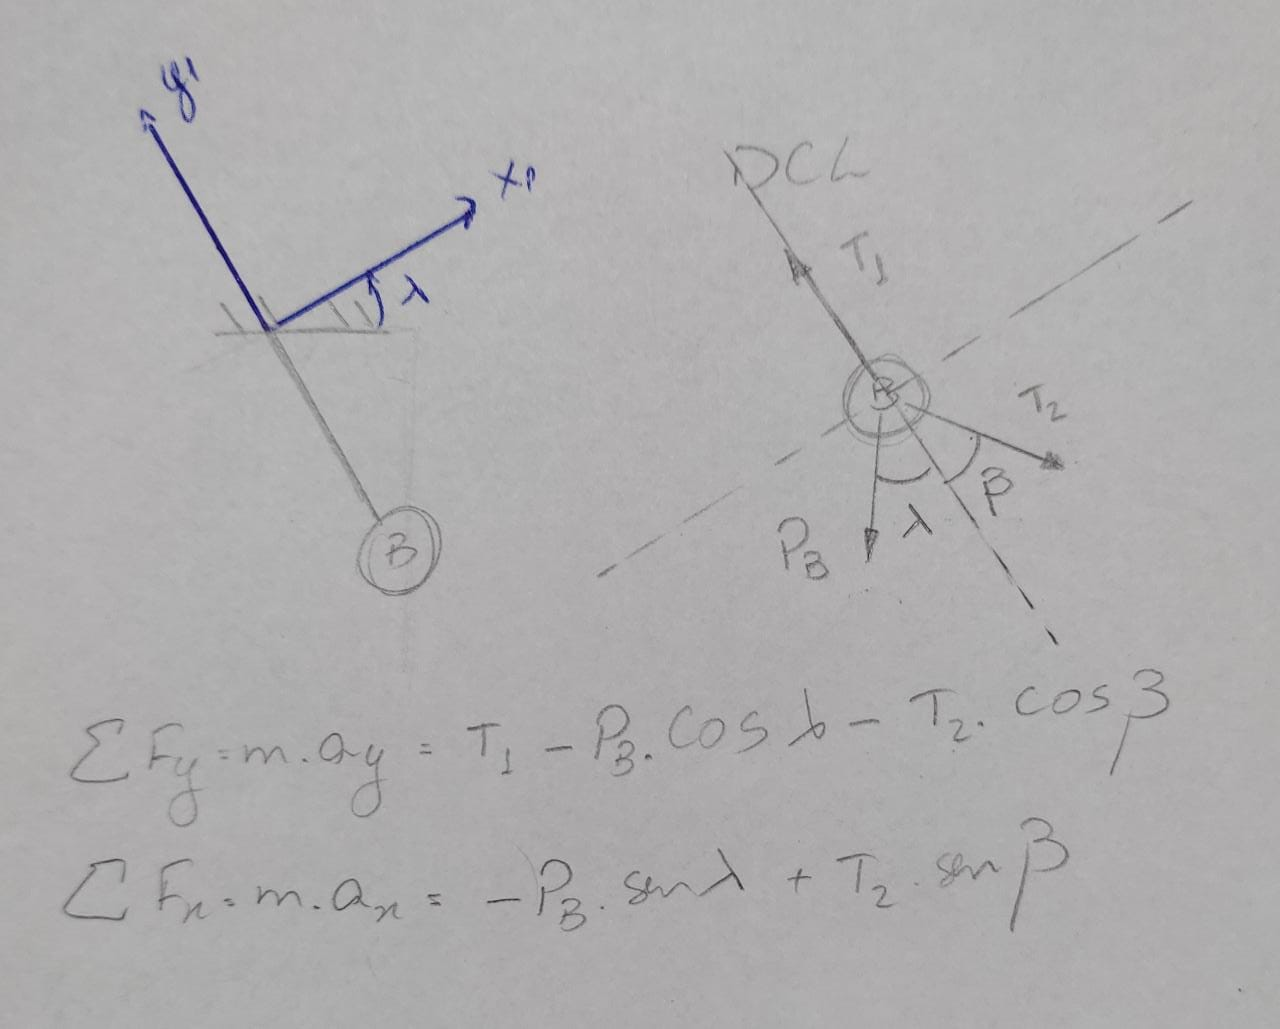
\includegraphics[scale=0.2]{a.jpg}
			\caption{Equilíbrio partícula B}
		\end{figure}
	\subsection{Partícula A}
		\begin{figure}[h]
			\centering
			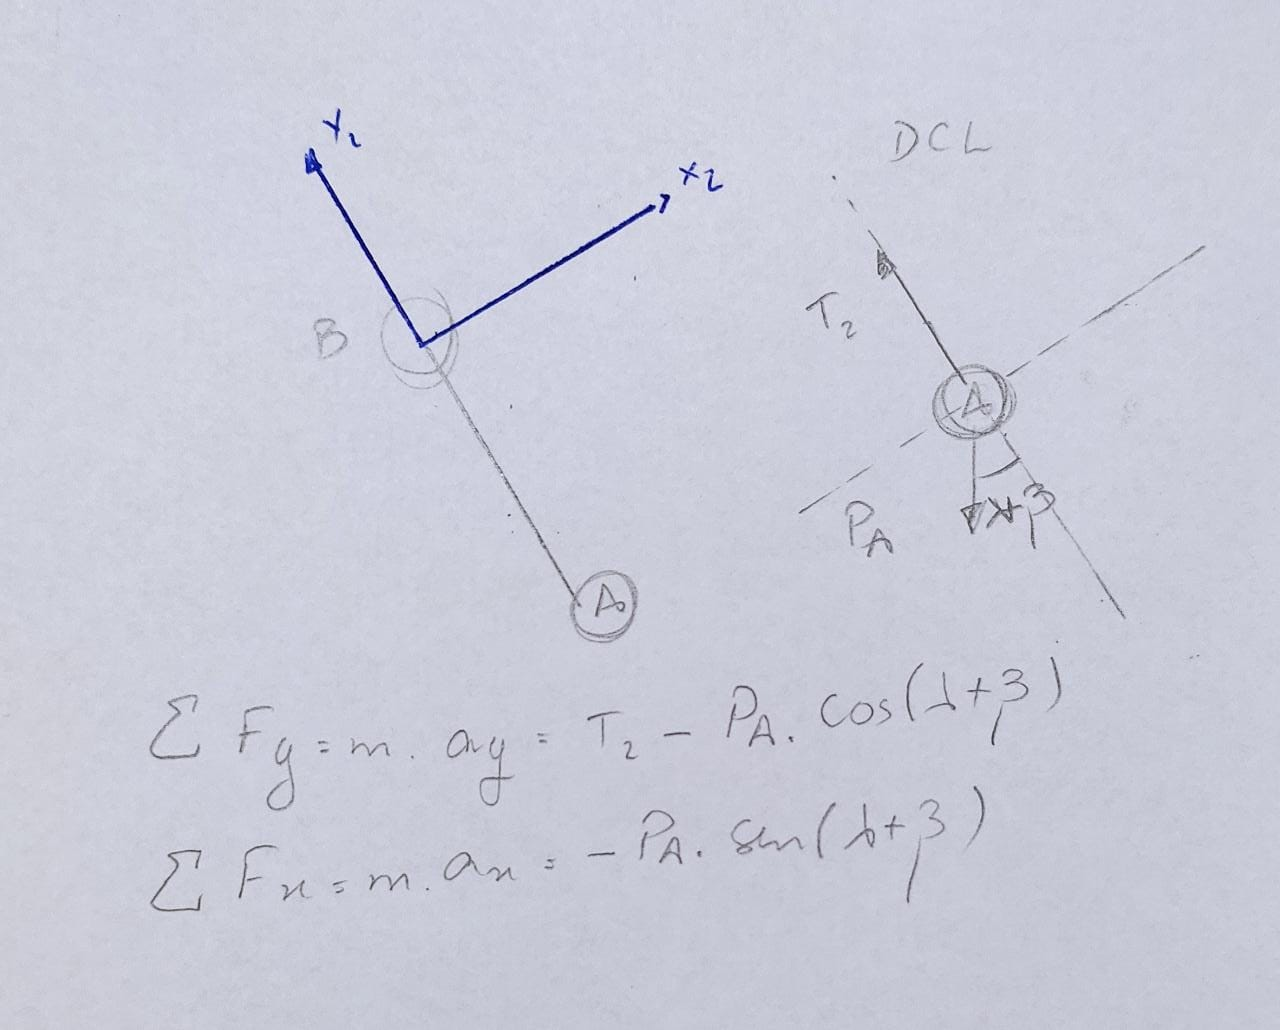
\includegraphics[scale=0.2]{b.jpg}
			\caption{Equilíbrio partícula A}
		\end{figure}

\newpage
\section{Método de Runge-Kutta}
	\begin{itemize}
		\item $m_1 = m_2 = 0.0046 kg$
		\item $l_1 = l_2 = 0.07m$
		\item $g = 9.81m/s^2$
		\item $\lambda(0) = -\pi/4$
		\item $\dot{\lambda}(0) = \dot{\beta}(0) = 0$
	\end{itemize}




\end{document}
